\chapter{Problem description and related work}

\label{ch:Problem description and related work}

\setlength{\parindent}{4em}
\setlength{\parskip}{1em}
\renewcommand{\baselinestretch}{1.5}

\section{Problem description}
\hspace{1.5cm} Nowadays, there are many people who have been born with a disabled body from various reasons. Most of them always have a limitation of their living that be different from ordinary people. At present, one of the main problems of the disabled person is lacking help and ignore from other people. Using knowledge from the scientific and engineering field to make a brain-computer interface machine is the way to help these people to have the living like the ordinary people. For our project, we decide to assist the patient or physically disabled people that can't completely move their body part to interaction without helping from other people such as Paralysis, Spinal cord injured, Stoke and ALS.

\section{Review of related works}
\subsection {Multitasking with BCI machine\cite{ref1}}
\hspace{1.5cm} The multitasking with BCI machine experiment from EPFL Professor José del R. Millan. This experiment develops the BCI machine which allows the user to control the robot direction to move by using EEG signal and real-time communicate with other people via the camera that mount on the robot.
\begin{figure}[ht]
	\centering
  	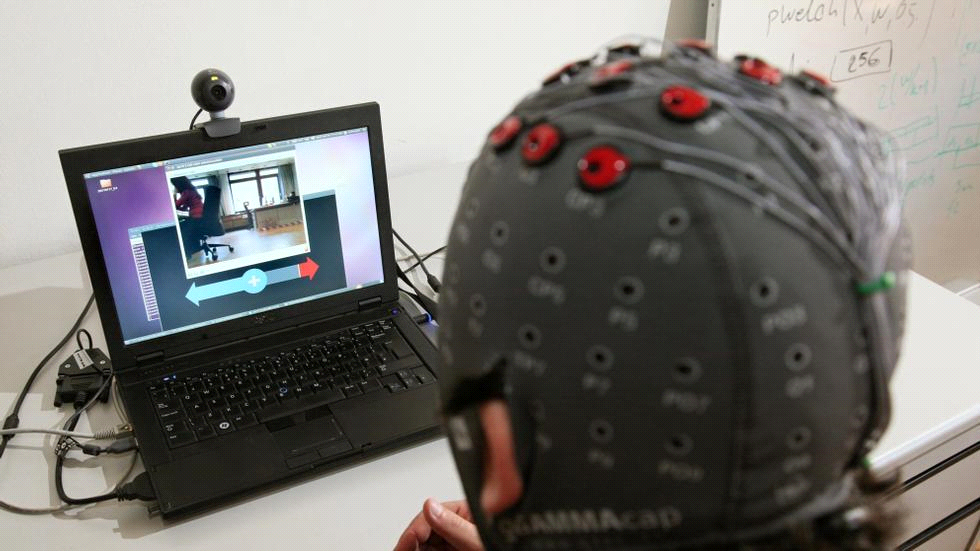
\includegraphics[scale = 0.4]{chapter2/21.png}
  	\caption{The subject control robot use brain wave and communicate via camera at same time}
\end{figure}

\subsection {Real-time control of a robotic arm using a brain-computer interface\cite{ref2}}

\hspace{1.5cm} SSVEP control of robotic arm experiment from the Applied Signal Processing in Engineering and Neuroscience Lab (ASPEN Lab) of Old Dominion University.\par
This Lab is used to develop an application which using EEG headset to control the robotic arm. The subject should gaze on the one of the flickers in front of him for control or command the direction of the robotic arm.
\begin{figure}[ht]
	\centering
  	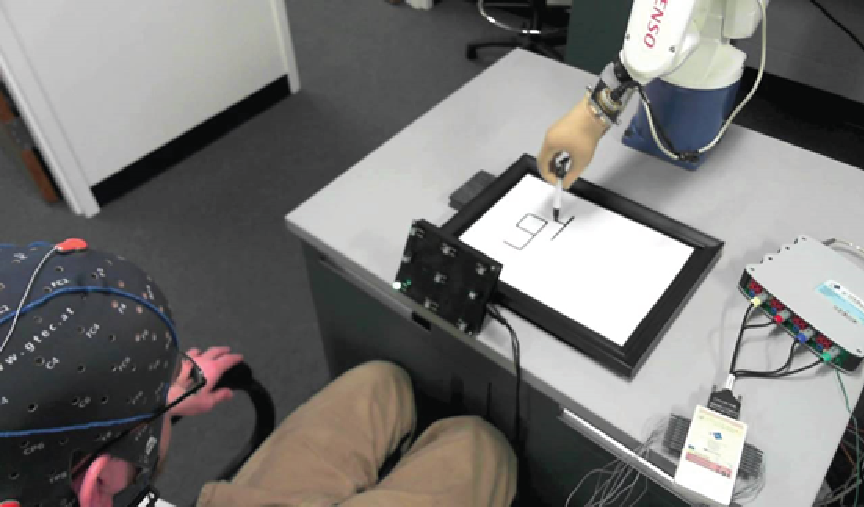
\includegraphics[scale = 0.70]{chapter2/22.pdf}
  	\caption{The subject control s robotic arm by fixate at stimulation ligth using SSVEP}
\end{figure}
\newpage

\subsection {Visual stimuli for the P300 brain-computer interface: A comparison of white/grey and green/blue flicker matrices\cite{ref3}}

\hspace{1.5cm}P300 speller has mainly used white/grey flicker matrices as visual stimuli but they are not reducing the fatigue condition of the user. Parra and colleagues evaluated what color is reducing the fatigue condition of the user. In their study, five single-color stimuli have been implemented. There are white, blue, red, yellow and green.\par
In this experiment, the green/blue chromatic flicker emerged as the safest and evoked the lowest rate of EEG spikes. The result showed that the accuracy rate was higher in response to the luminance chromatic flicker condition(LC) than in response to the luminance(L) or chromatic(C) flicker condition.\par
In conclusion, most users preferred green and blue make them feel less strain on the eyes. The subjects found that they could use green stimulus for longer periods as compared with red and blue in all frequency range.

\begin{figure}[ht]
	\centering
  	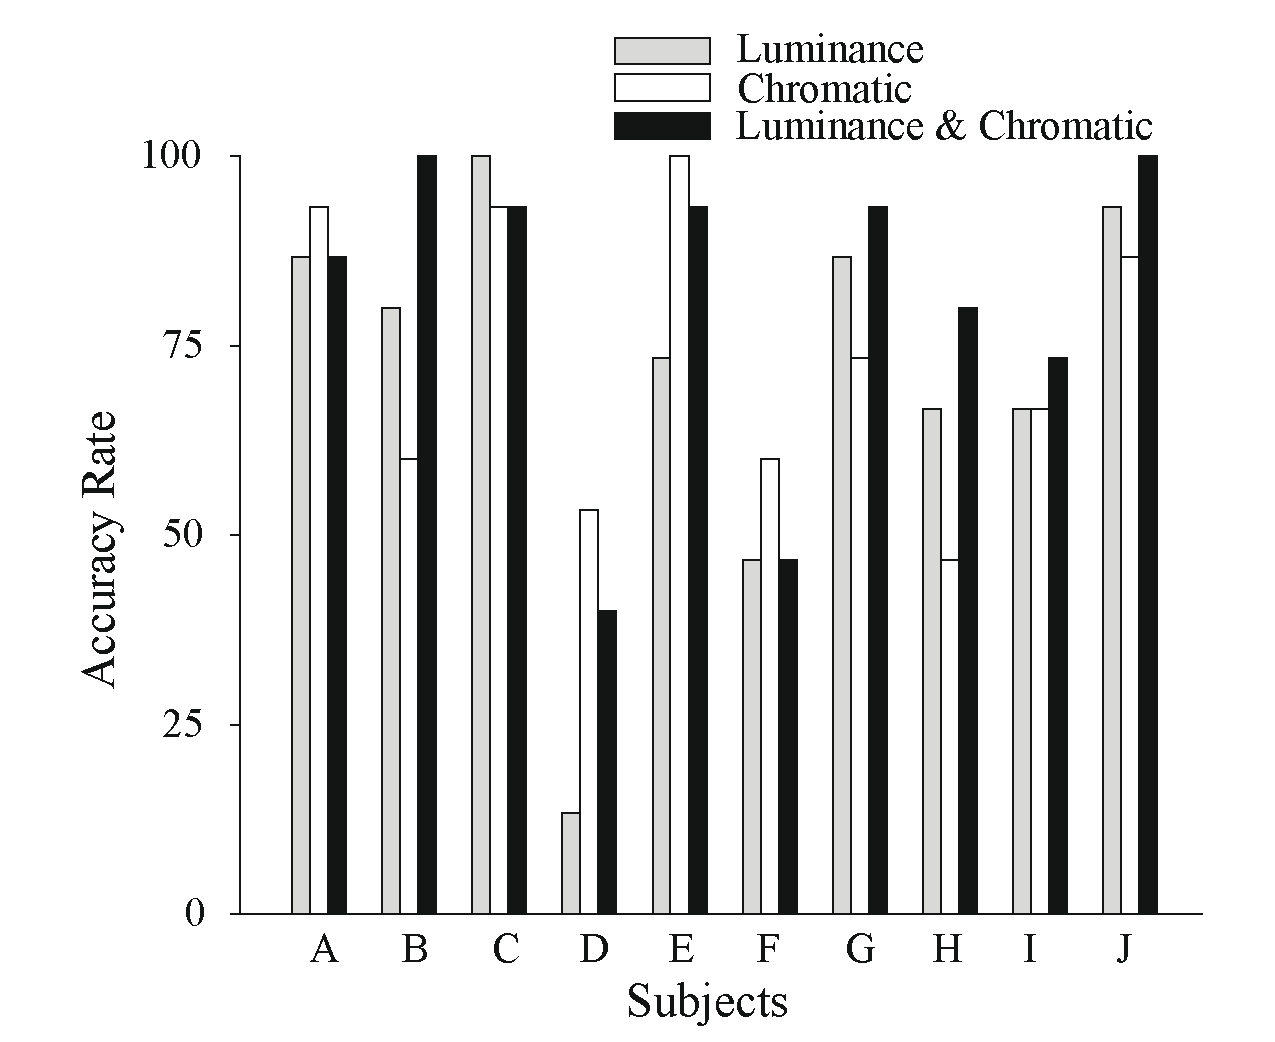
\includegraphics[scale = 0.5]{chapter2/23.pdf}
  	\caption{Accuracy rates for each subject. The accuracy rates in L, C, and LC conditions for each subject (A–J) are indicated by grey bars, white bars, and black bars, respectively.}
\end{figure}

\newpage
\subsection {Validation of the Emotiv EPOC® EEG gaming system for measuring research quality auditory ERPs\cite{ref4}}
\hspace{1.5cm} There are two kinds of equipment for obtaining a brain signal as follow: Researching headset and Gaming headset. Studying this research can be concluded that the Gaming headset can be use as well as the Research headset because of the result of an experiment showed that the characteristics of the Gaming headset's graph are very similar to the graph of Research headset.

\begin{figure}[ht]
	\centering
  	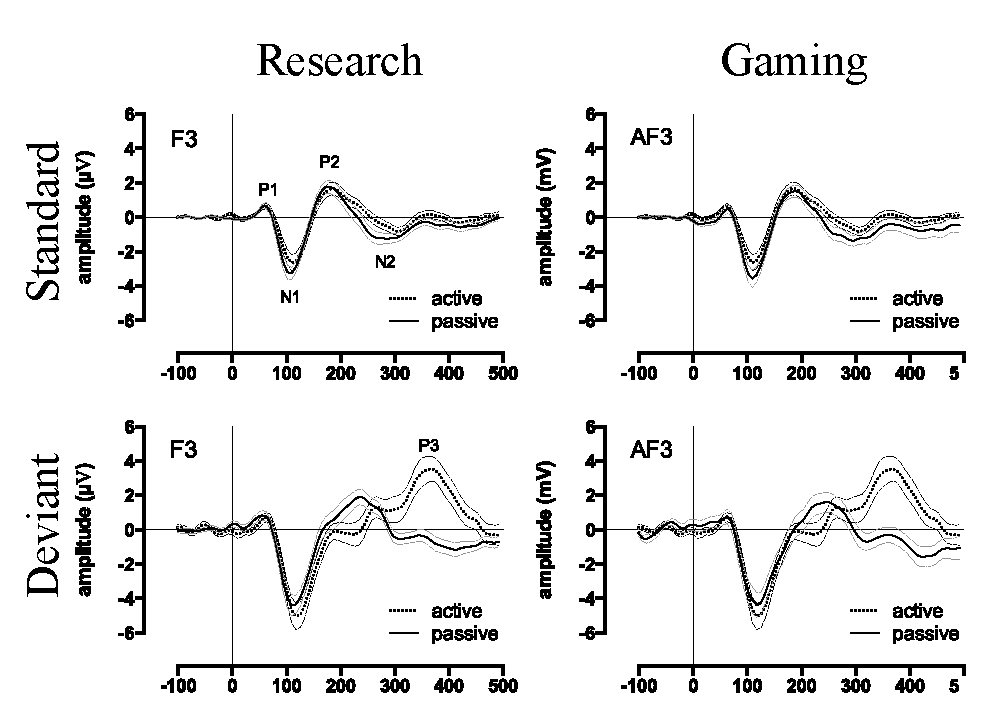
\includegraphics[scale = 0.75]{chapter2/24.pdf}
  	\caption{Research and gaming system ERP waveform by condition, tone type, and hemisphere. Group ERP waveform for research (left-side) and gaming (right-side) systems. All graphs display waveform for the passive and active (counting deviant tones) listening conditions. The upper 4 graphs depict the left-hemisphere-activity (F3 and AF3) and the lower 4 graphs depict the right-hemisphere-activity (F4 and AF4). Rows 1 and 3 depict waveform elicited by the standard tones, rows 2 and 4 depicts waveform elicited by the deviant tones. Error waveform (in gray) represent the standard error of the mean. For  passive and active (counting deviant tones) listening conditions}
\end{figure}
\newpage

\subsection {c-VEP Brain-Computer Interface (BCI)\cite{ref5}}

\hspace{1.5cm} Code-modulated visual evoked potentials (c-VEP) is one of the kinds of BCI. c-VEP uses pseudorandom code to modulate different visual stimuli. The figure 2.5 A shows the configuration and modulation of the c-VEP BCI system

\begin{figure}[ht]
	\centering
  	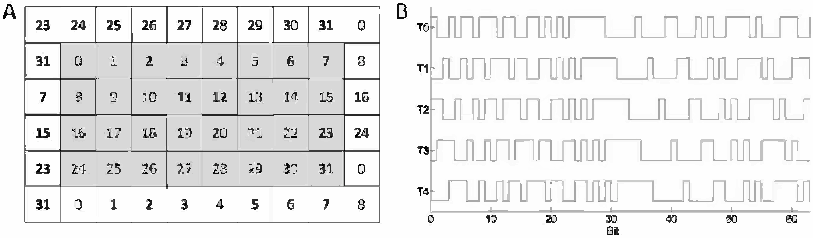
\includegraphics[scale = 1]{chapter2/25.pdf}
  	\caption{A: The gray area shows the 32 target stimuli with the number referring to number of  target. The stimuli in white area are the complementary, which are synchronized to the target with same number. B: Modulation sequence for the first 5 targets. The sequence of a target is shifted by 2 bit in respect to its preceding target.}
\end{figure}

\subsection {SSVEP-based brain computer interface using the Emotiv EPOC\cite{ref6}}

\hspace{1.5cm} After the data was obtained from the headset, the two occipital channels were averaged together which help eliminated some noise between two channels. Because SSVEP is base on a particular frequency being present in the EEG data, the signal processing should be accomplished by using a Fourier transform to convert from the time domain into the frequency domain. 
After averaged the data, The result from converting is a frequency spectrum. Then, squaring the amplitude of each frequency component in this spectrum. This result was collected as active signal spectrum After that using a baseline removal method to further improve the results of signal isolation for the identification of SSVEP response. A baseline was recorded while the user was viewing a solid 50 percent gray screen without present any visual stimulation. After the data was recorded, Begin the method by using a Fourier transform with baseline spectrum and then reduce the noise by using a smoothing filter. Finally, the smoothed baseline spectrum was subtracted from the active signal spectrum. Finally, the result from this is the spectrum that can classify the observed data.\\ 

\begin{figure}[ht]
	\centering
	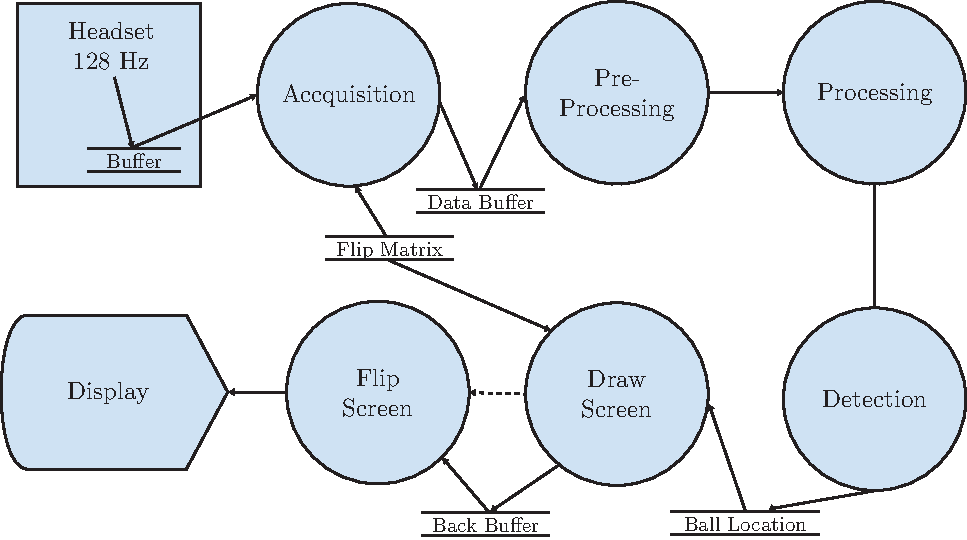
\includegraphics[scale = 0.8]{chapter2/29.pdf}
	\caption{Diagram of data processing in EEG headset device \cite{ref6}}
\end{figure}

\subsection {A Survey of Stimulation Methods Used in SSVEP-Based BCIs\cite{ref7}}

\hspace{1.5cm} The stimulus frequency can be divided into three bands. that is low (1-12 Hz), medium (12-30 Hz) and high (30-60 Hz). The largest SSVEP amplitudes were observed near 10 Hz followed by 16-18 Hz. Therefore, the most of the SSVEP-based BCIs use low and medium frequency bands. However, These two frequency bands have the disadvantage. First, the subjective evaluation shows that frequency between 5 and 25 Hz are more annoying than higher ones which visual fatigue would easily occur. Second, flash and pattern reversal stimuli can provoke epileptic seizures especially in the 15-25 Hz range. Third, the low-frequency band covers the alpha band (8-13 Hz) which can cause a considerable amount of false positives. All of these disadvantages can be avoided by using the higher frequency band.  

\begin{figure}[ht]
	\centering
	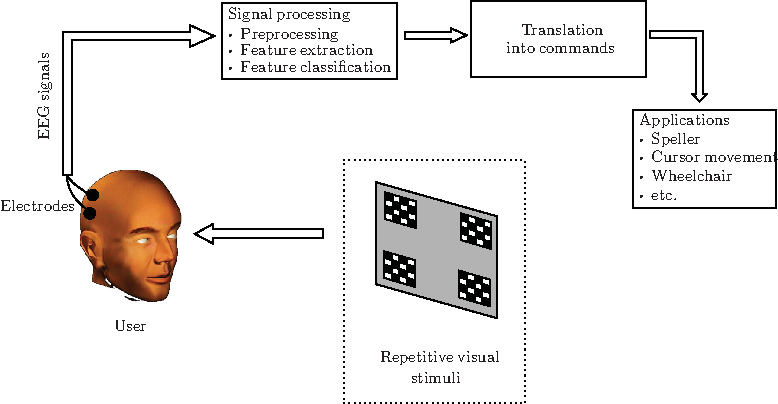
\includegraphics[scale = 1.2]{chapter2/210.pdf}
	\caption{ Functional model of an SSVEP-based BCI}
\end{figure}  

\newpage
\subsection {Human EEG responses to 1-100 Hz flicker\cite{ref8}}

\hspace{1.5cm} Human EEG responses to 1-100 Hz flicker is stimulated in visual cortex. Herrmann reported that the SSVEP responses exhibited resonance phenomena around 10,20,40 and 80 Hz

\begin{figure}[ht]
	\centering
  	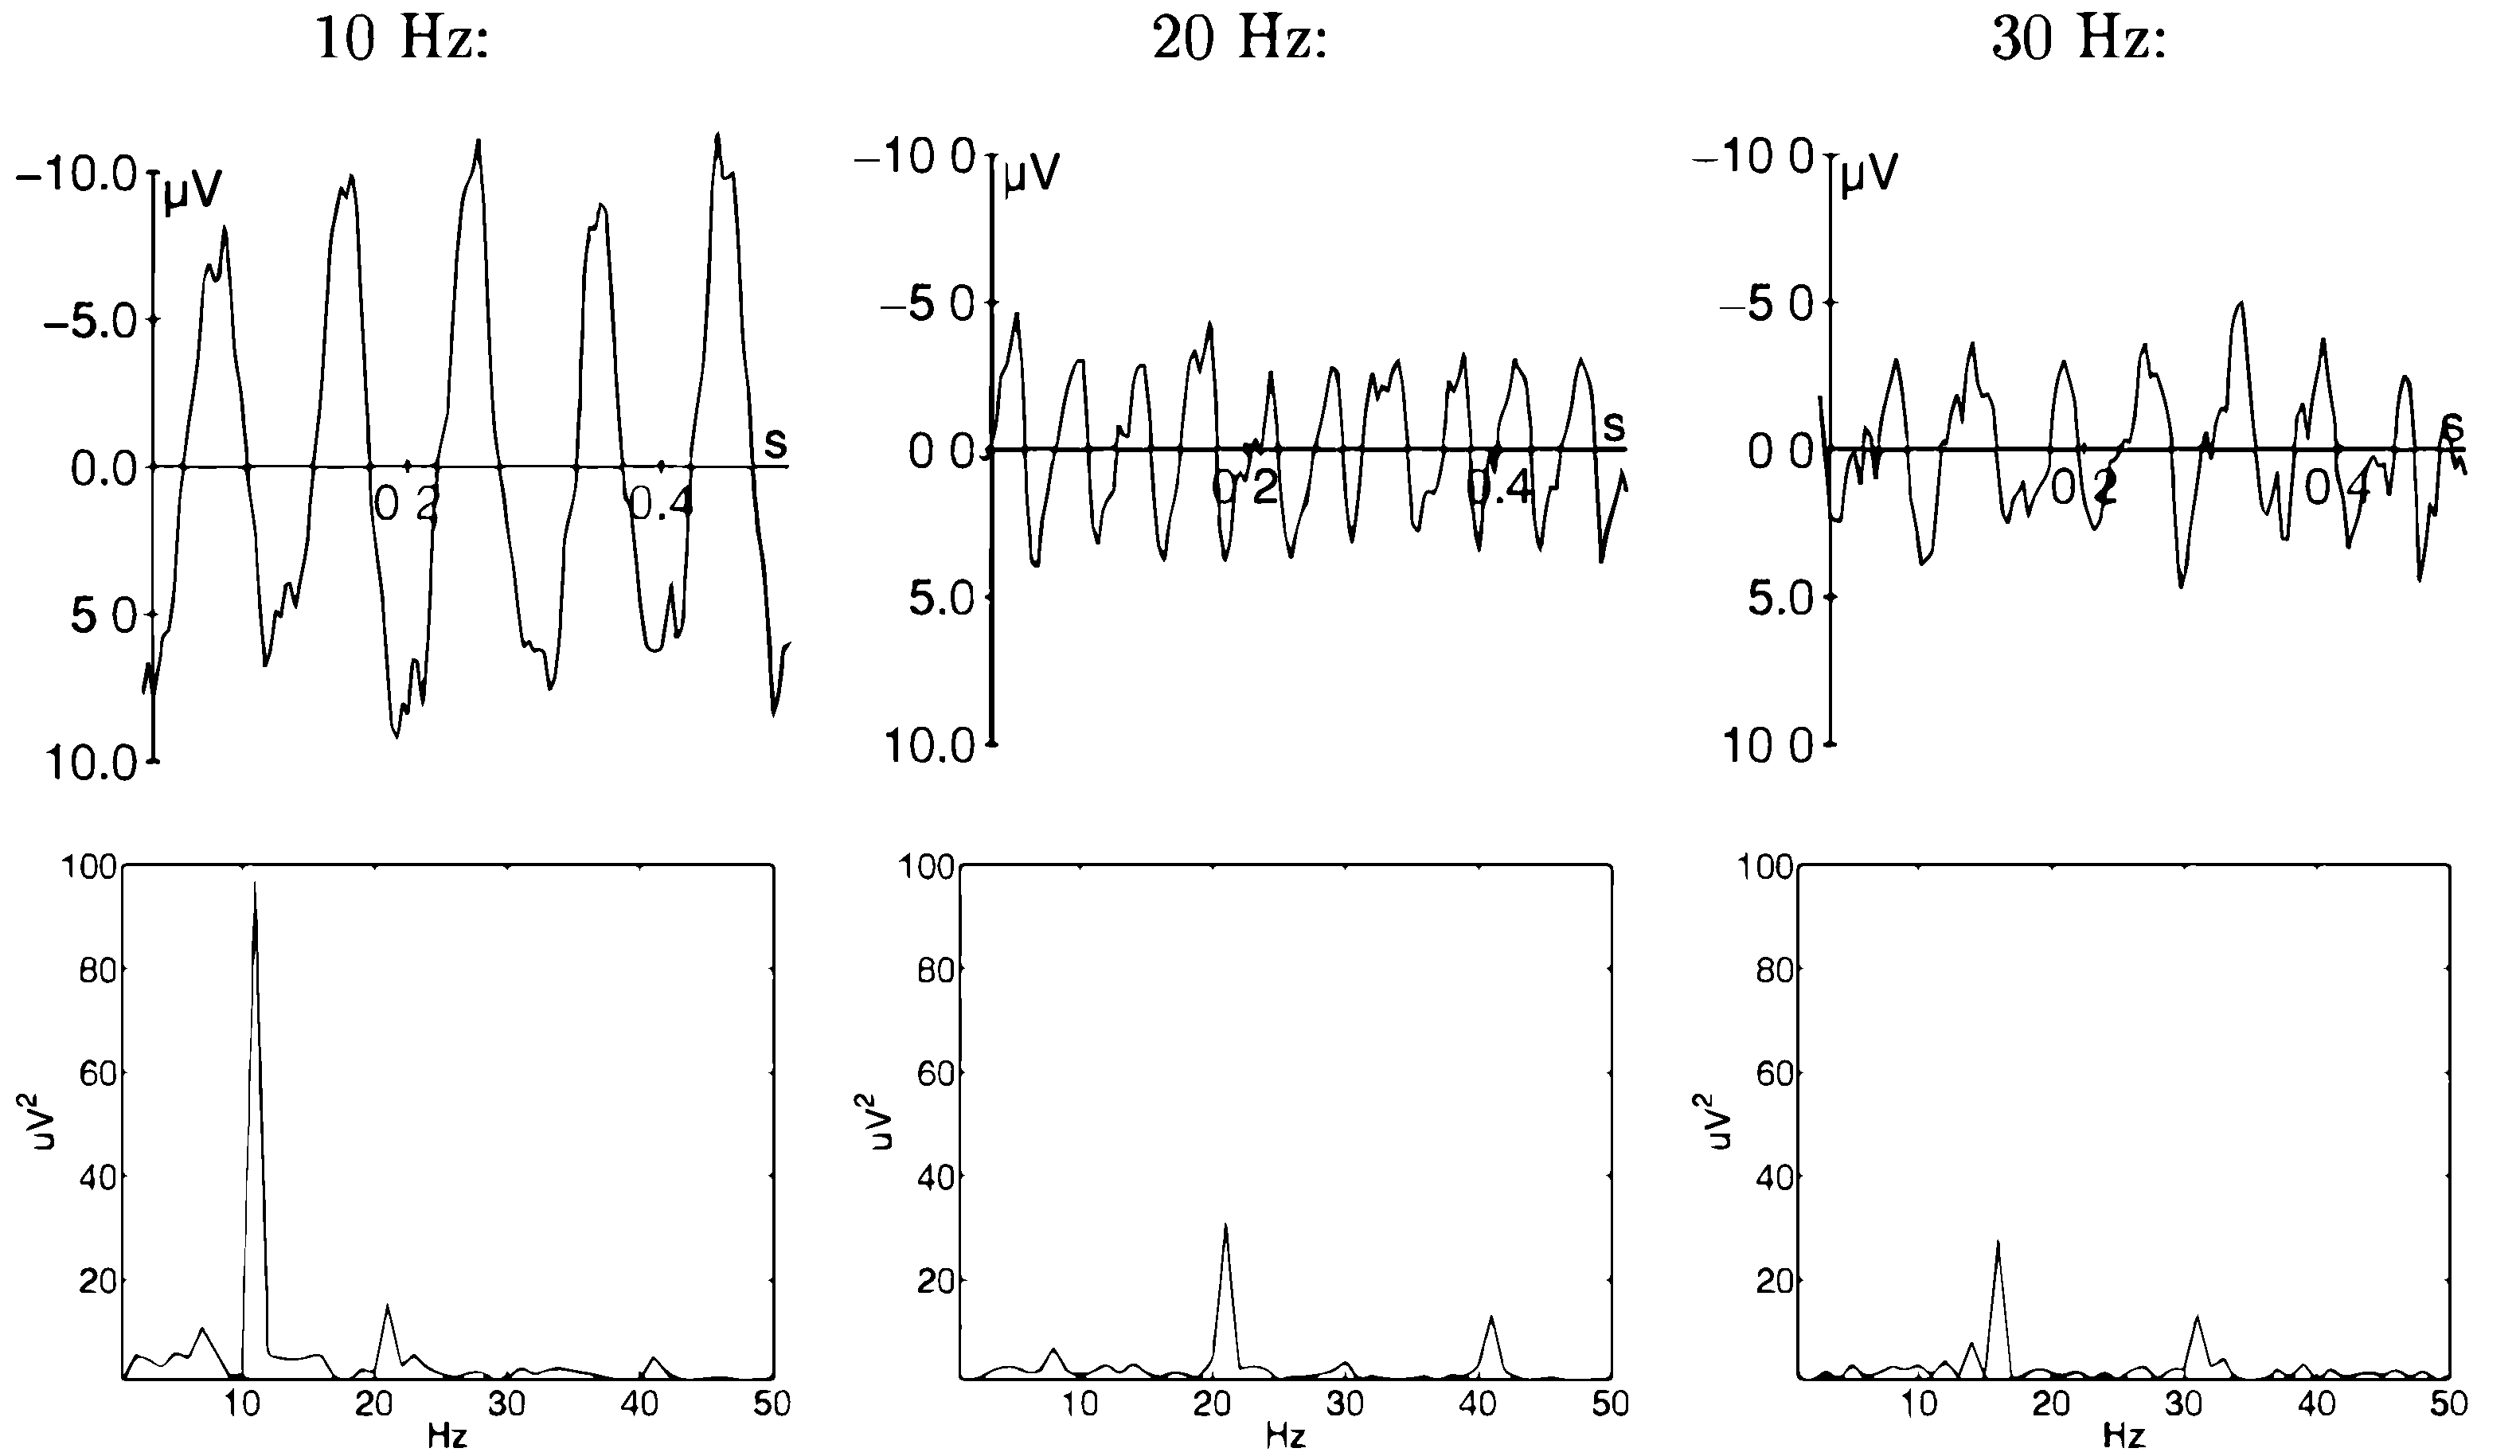
\includegraphics[scale = 0.21]{chapter2/26.pdf}
  	\caption{SSVEPs of a single subject in response to 10 Hz (left), 20 Hz (middle) and 30 Hz (right) stimulation (top row) and the corresponding FFT frequency spectra (bottom row)}
\end{figure}

\begin{figure}[ht]
	\centering
  	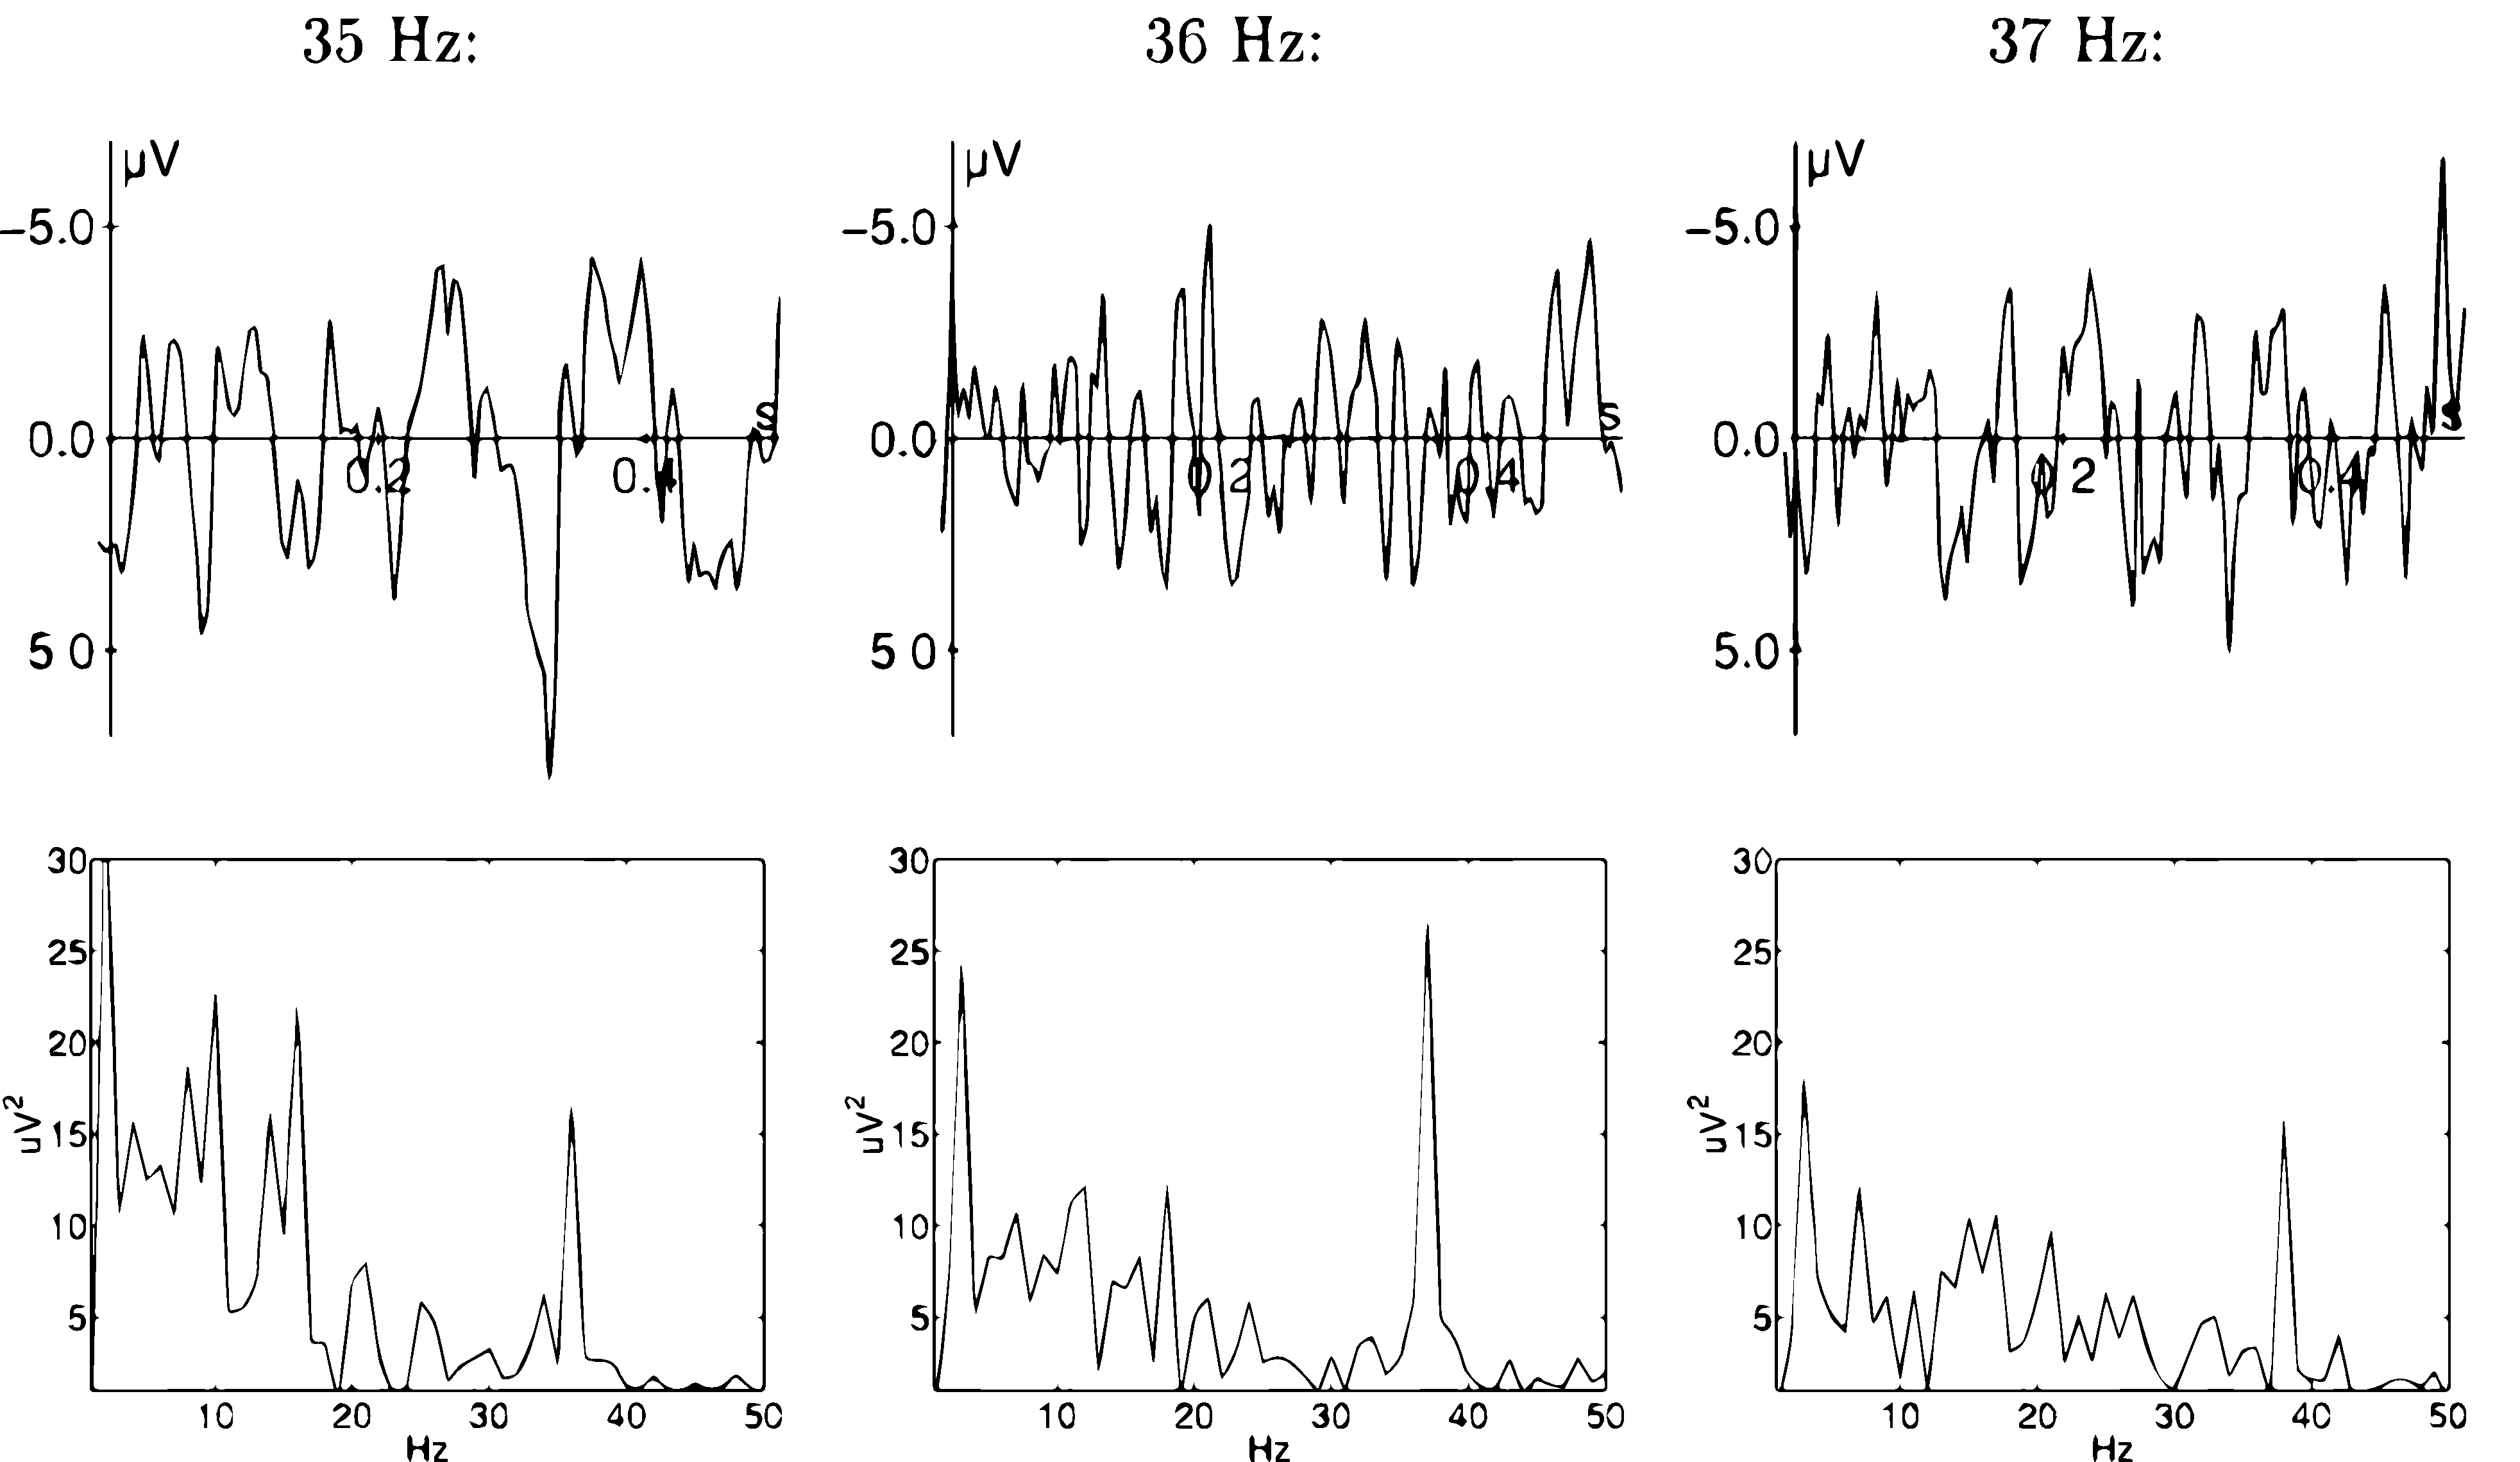
\includegraphics[scale = 0.2]{chapter2/27.pdf}
  	\caption{SSVEPs of a single subject in response to 35 Hz (left), 36 Hz (middle) and 37 Hz (right) stimulation (top row). The corresponding FFT frequency spectra show an increase of power at 36 Hz for 36 Hz stimulation (middle) as compared to adjacent frequencies (left and right)}
\end{figure}

\begin{figure}[ht]
	\centering
  	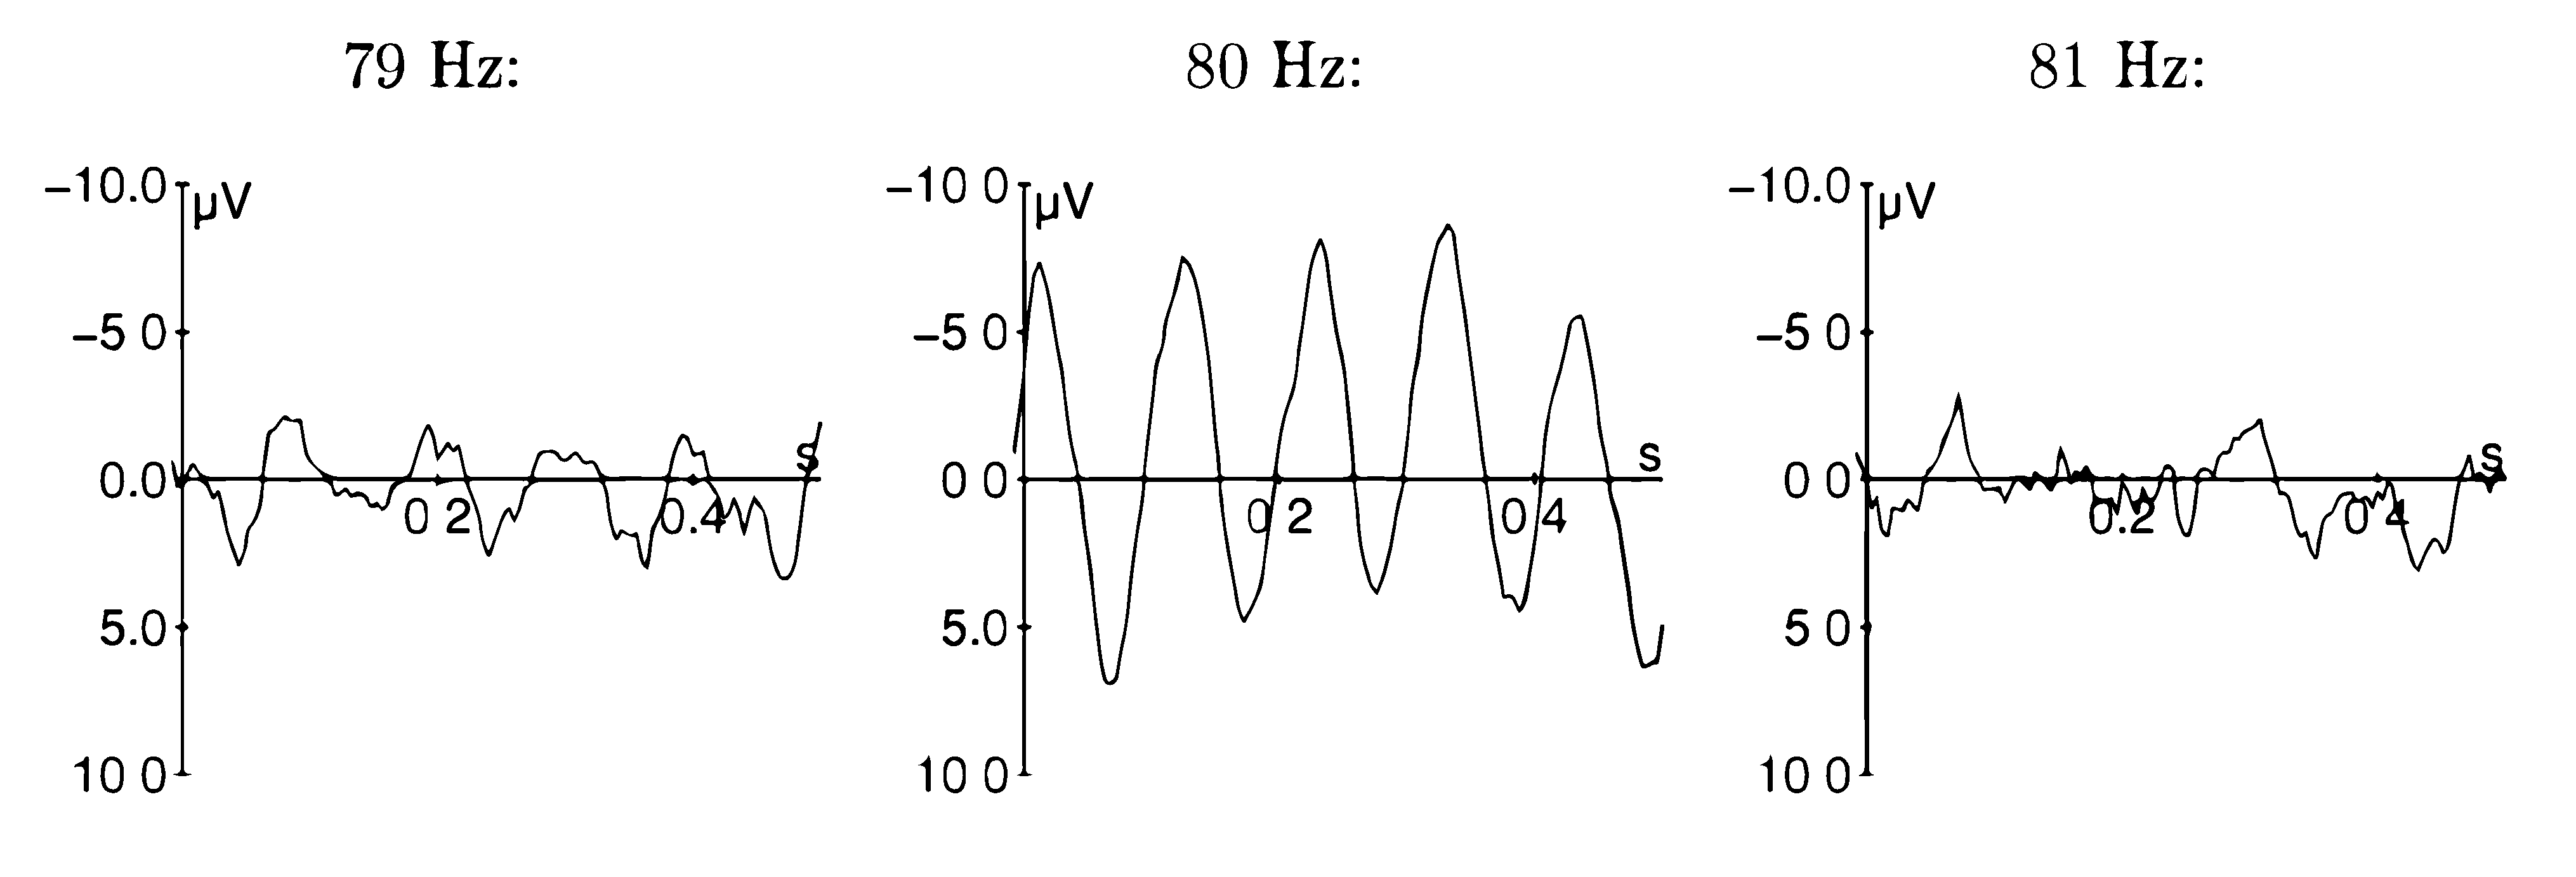
\includegraphics[scale = 0.18]{chapter2/28.pdf}
  	\caption{ SSVEPs in response to flicker frequencies 79 (left), 80 Hz (middle) and 81 Hz (right). The VEP shows clear 10-Hz oscillations at 80 Hz which are not as prominent for the adjacent frequencies}
\end{figure}

\subsection {Effect of higher frequency on the classification of steady-state visual evoked potentials\cite{ref7}}

\hspace{1.5cm}This research developed an SSVEP-based BCI speller using multiple LEDs flickering with low frequencies (6 to 14.9 Hz) with a duty-cycle of 50 percent, or higher frequencies (26 to 34.7 Hz) with duty-cycles of 50 percent, 60 percent, and 70 percent. The four different experimental conditions were tested with 26 subjects in order to investigate the impact of stimulation frequency and duty-cycle on visual fatigue by evaluated with a questionnaire survey after they did the experiment.The questionnaire used a five level satisfaction rating score of ‘1 : unacceptable’, ‘2 : uncomfortable’, ‘3 : acceptable’, ‘4 : comfortable’, and ‘5 : delightful’.


